\section{Evaluation}
\label{sec:eval}

We now evaluate preemptible function performance, presenting several
microbenchmarks and two examples of their application to improve
existing systems' resilience to malicious or otherwise long-running
requests.  All experiments were run on an Intel Xeon E5-2683 v4 (Broadwell)
server running Linux 4.12.6, rustc 1.36.0, gcc 9.2.1, and glibc 2.29.

\solb{Should we mark every test we run without global variable interposition?}


\subsection{Microbenchmarks}

\begin{table}
\begin{center}
\begin{tabular}{c | c}
Operation & Duration ($\mu{s}$) \\
\hline
\texttt{launch()} & $4.6 \pm 0.05$ \\
\texttt{resume()} & $4.4 \pm 0.02$ \\
\texttt{cancel()} & $4767.7 \pm 1168.7$ \\
\hline
\texttt{fork()} & $207.5 \pm 79.3$ \\
\texttt{pthread\_create()} & $32.5 \pm 8.0$
\end{tabular}
\end{center}
\caption{Latency of preemptible function interface}
\solb{Rerun with the latest version of libinger.}
\label{tab:libinger}
\end{table}

Table~\ref{tab:libinger} shows the overhead of \textit{libinger}'s core functions.
Each test uses hundreds of preemptible functions, each with its own stack and
continuation, but sharing an implementation; the goal is to measure invocation time,
so the function body immediately calls \texttt{pause()}.
For comparison, we also measured the cost of calling \texttt{fork()} then
\texttt{exit()}, and of calling \texttt{pthread\_create()} with an empty function,
while the parent
thread waits using \texttt{waitpid()} or \texttt{pthread\_join()}, respectively.

The results show that, as long as preemptible functions are eventually allowed to run
to completion, they are an order of magnitude faster than spawning a thread and two
orders of magnitude faster than forking a process.  Although cancellation takes
milliseconds in the benchmark application, this operation need not lie on the
critical path unless the application is cancelling tasks frequently enough to exhaust
its supply of libsets.

\begin{table*}
	\begin{minipage}{2\columnwidth}
	\centering
	\begin{tabular}{c | c c}
	Symbol resolution scheme & Time without \textit{libgotcha} ($ns$) & Time with \textit{libgotcha} ($ns$) \\
	\hline
	eager (load time) & $2 \pm 0$ & $14 \pm 0$ \\
	lazy (runtime) & $100 \pm 1$ & $125 \pm 0$ \\
	global variable & $0 \pm 0$ & $3438 \pm 13$
	\end{tabular}
	\subcaption{Generic symbols, with and without \textit{libgotcha}}
	\label{tab:libgotcha:symb}
	\end{minipage}

	\begin{minipage}{\columnwidth}
	\centering
	\begin{tabular}{c | c}
	Baseline & Time without \textit{libgotcha} ($ns$) \\
	\hline
	\texttt{gettimeofday()} & $19 \pm 0$ \\
	\texttt{getpid()} & $44 \pm 0$
	\end{tabular}
	\subcaption{Library functions and syscalls without \textit{libgotcha}}
	\label{tab:libgotcha:baseline}
	\end{minipage}
%
	\begin{minipage}{\columnwidth}
	\centering
	\begin{tabular}{c | c}
	Trigger & Time with \textit{libgotcha} ($ns$) \\
	\hline
	Uninterruptible call & $21 \pm 0$ \\
	Uninterruptible call + callback & $25 \pm 0$
	\end{tabular}
	\subcaption{Uninterruptible calls triggering a libset switch}
	\label{tab:libgotcha:whitelist}
	\end{minipage}
\caption{Runtime overheads of accessing dynamic symbols}
\end{table*}

Recall that linking an application against \textit{libgotcha} imposes additional
overhead on every dynamic symbol access; we report these overheads in
Table~\ref{tab:libgotcha:symb}.  Eager function calls account for almost all of a
modern program's dynamic symbol accesses:  Direct access to global variables is rarer
now that thread safety is a pervasive concern, with libc removing the \texttt{errno}
symbol in favor of an \texttt{\_\_errno\_location()} helper
function~\cite{www-lsb-errno}, and compilers now translating thread-local variable
accesses into calls to \texttt{\_\_tls\_get\_addr()} or offsets from a segment
register~\cite{drepper:spec2013}.  As explained in Section~\ref{sec:libgotcha}, lazy
resolution only occurs the first time an object file calls a particular function, and
it can be avoided altogether by asking the dynamic linker to resolve all symbols at
load time.

Table~\ref{tab:libgotcha:baseline} shows that the \textit{libgotcha} eager function
call overhead of 14 ns is on par with the cost of a trivial C library function and
one-third
that of a simple system call.  This overhead affects the entire program, regardless
of the
current libset at the time of the call.  Additionally, calls to
uninterruptible functions from within a preemptible function incur several extra
nanoseconds of latency to switch back to the main namespace as described in
Section~\ref{sec:libgotcha}; Table~\ref{tab:libgotcha:whitelist} breaks this down to
show the cost of notification callbacks at the conclusion of such a call (always
required by \textit{libinger}).


\subsection{Web server}

To test whether our thread library could combat head-of-line blocking in a large
system, we benchmarked
\textit{hyper}, the highest-performing Web server in TechEmpower's plaintext
benchmark as of July 2019~\cite{www-hyper}.  We built \textit{hyper} against
\textit{libturquoise} configured with a task timeout of 2 ms, give or take a
100-$\mu$s \textit{libinger} preemption interval, and configured it to serve
responses only after spinning in a busy loop for a number of iterations specified in
each request.  For our client, we modified version 4.1.0 of the
\textit{wrk}~\cite{www-wrk} closed-loop HTTP load generator to separately record the
latency distributions of two different request classes.

Our testbed consisted of two machines connected by a direct 10-GbE link.  We pinned
\textit{hyper} to the 16 physical cores on the NIC's NUMA node of our Broadwell
server.  Our client machine, a Intel Xeon E5-2697 v3 (Haswell) running Linux 4.10.0,
ran a separate \textit{wrk} process pinned to each of the 14 logical cores on the
NIC's NUMA node.  Each client core maintained two concurrent pipelined HTTP
connections.

\begin{figure*}
	\begin{minipage}{\columnwidth}
	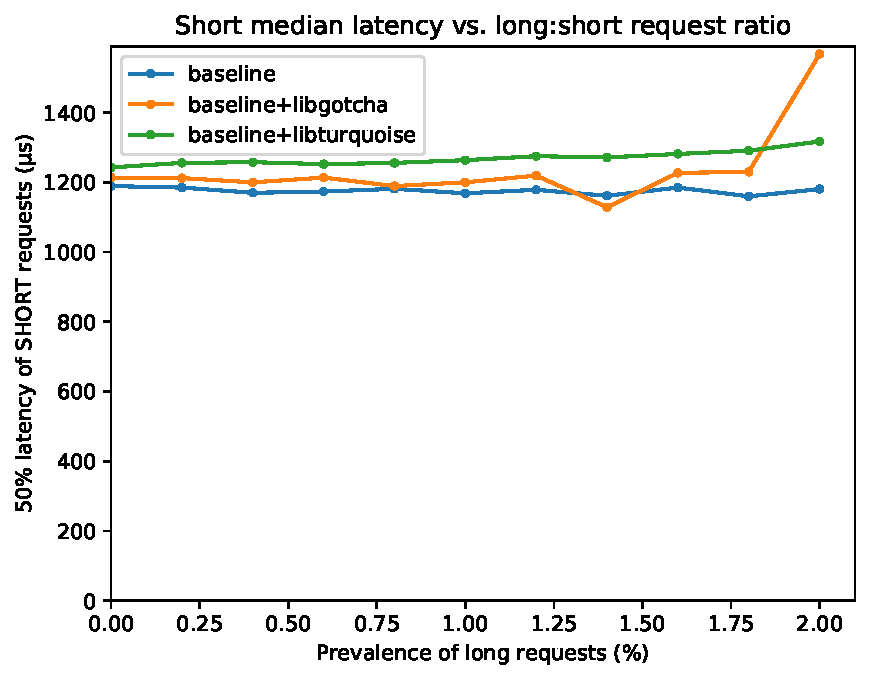
\includegraphics[width=\textwidth]{figs/twooom_50-short}
	\subcaption{Median latency}
	\end{minipage}
%
	\begin{minipage}{\columnwidth}
	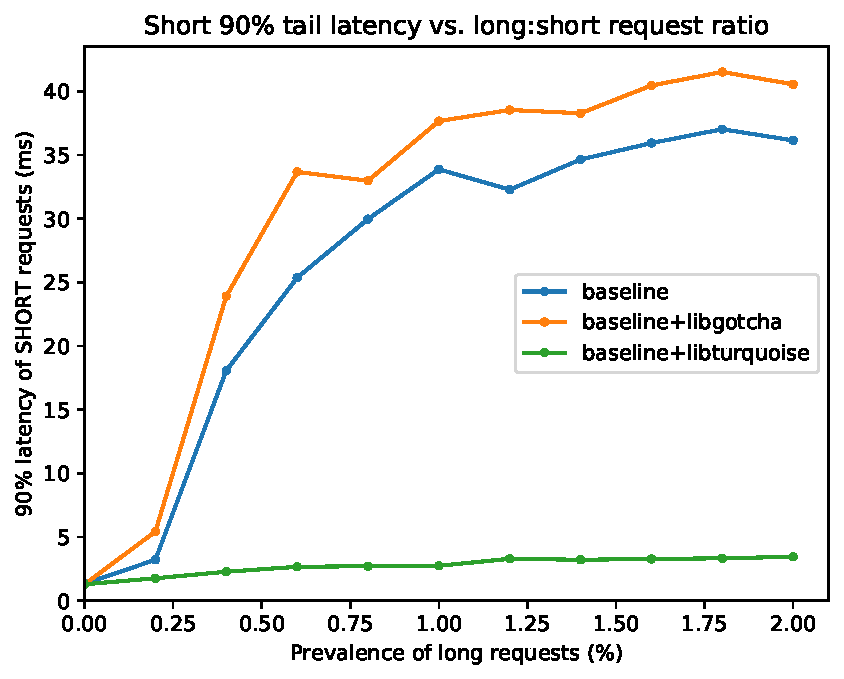
\includegraphics[width=\textwidth]{figs/twooom_90-short}
	\subcaption{90\% tail latency}
	\end{minipage}

	\begin{minipage}{\columnwidth}
	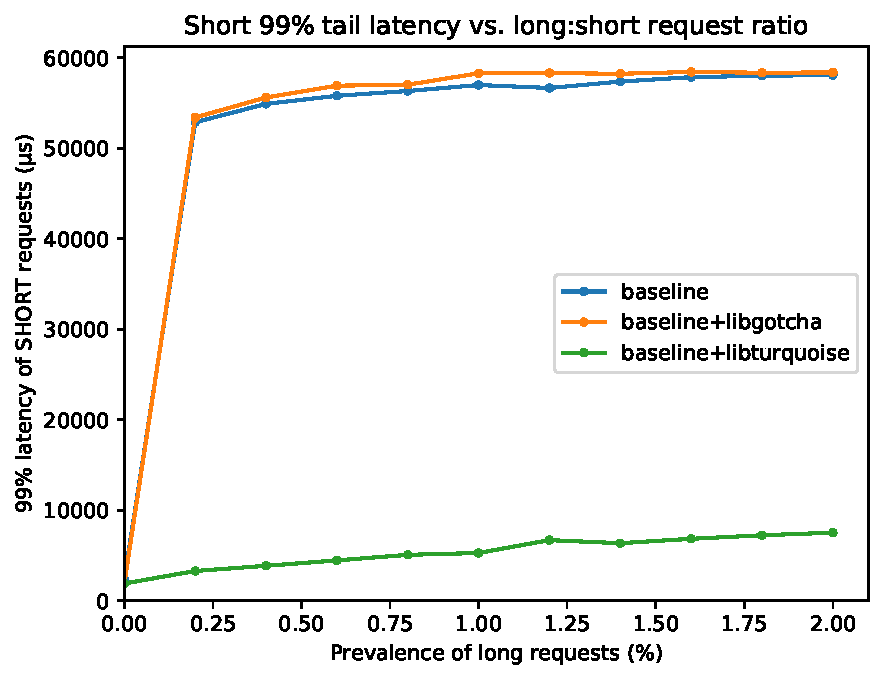
\includegraphics[width=\textwidth]{figs/twooom_99-short}
	\subcaption{99\% tail latency}
	\end{minipage}
%
	\begin{minipage}{\columnwidth}
	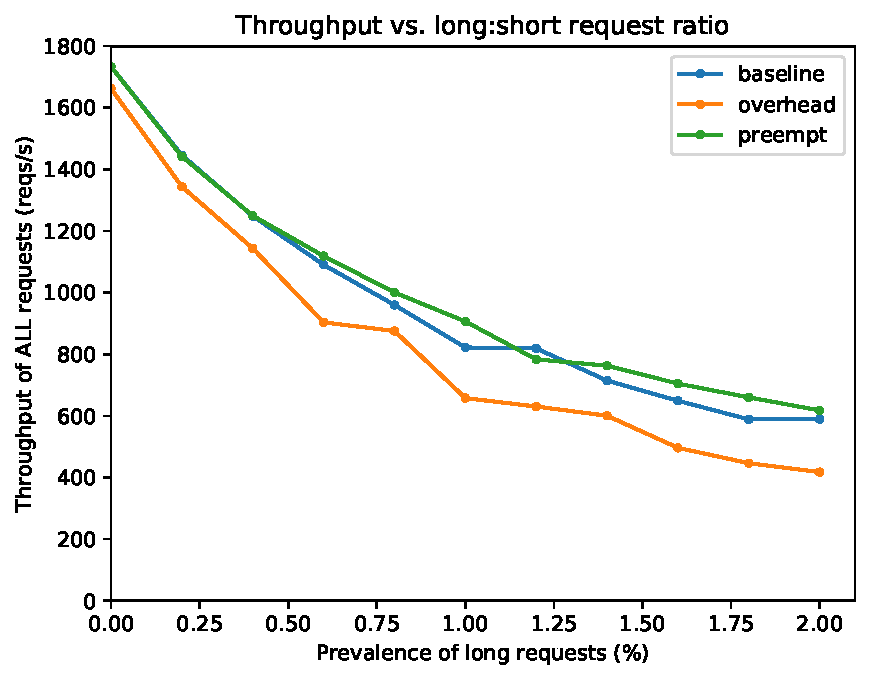
\includegraphics[width=\textwidth]{figs/twooom_tput}
	\subcaption{Overall throughput}
	\end{minipage}
\caption{\textit{hyper} Web server with 500-$\mu$s (short) and 50-ms (long) requests}
\label{fig:hyper}
\end{figure*}

We used loop lengths of approximately 500 $\mu$s and 50 ms for short and long requests,
respectively, viewing the latter requests as possible DoS attacks on the system.
We varied the percentage of long requests from 0\% to 2\% and measured the round-trip
median and tail latencies of short requests and the throughput of all requests.
Figure~\ref{fig:hyper} plots the results for three server configurations:\@
\texttt{baseline} is cooperative scheduling via \textit{tokio-threadpool},
\texttt{baseline+libgotcha} is the same but with \textit{libgotcha} loaded to assess
the
impact of slower dynamic function calls, and \texttt{baseline+libturquoise} is
preemptive
scheduling via \textit{libturquoise}.  The experiment shows that the preemptible
functions stack keeps the tail latency of short requests scaling linearly at the cost
of a
modest 4.5\% median latency overhead when not under attack.

\solb{Is it worth trying to get this running with HTTPS to increase dependence on
dynamic libraries?}


\subsection{Image decompression}

The Web benchmark showed preemptive scheduling at scale, but does not exercise
preemptible function cancellation.  To demonstrate this feature, we consider
decompression bombs, files that expand exponentially when decoded, consuming enormous
computation time in addition to their large memory footprint.
PNG files are vulnerable to such an attack, and although \textit{libpng} now
supports some mitigations~\cite{www-libpng-bombs}, one cannot always expect (or
trust) such functionality from a third-party codec.

We benchmarked the use of \textit{libpng}'s ``simple API'' to decode an in-memory PNG
file.  We then compared against synchronous isolation using preemptible functions, as
well as the na\"ive alternative mitigations proposed in Section~\ref{sec:intro}.  For
preemptible functions, we wrapped all uses of \textit{libpng} in a call to
\texttt{launch()} and used a dedicated (but blocking) reaper thread to remove the
cost of cancellation from the critical path; for threads, we used
\texttt{pthread\_create()} followed by \texttt{pthread\_timedjoin\_np()} and a
conditional \texttt{pthread\_cancel()} (with asynchronous cancelability enabled); and
for processes, we used \texttt{fork()} followed by \texttt{sigtimedwait()}, a
conditional \texttt{kill()}, then a \texttt{waitpid()} to reap the child.  We used a
timeout of 10 ms in all cases.

\begin{figure*}
	\begin{minipage}{\columnwidth}
	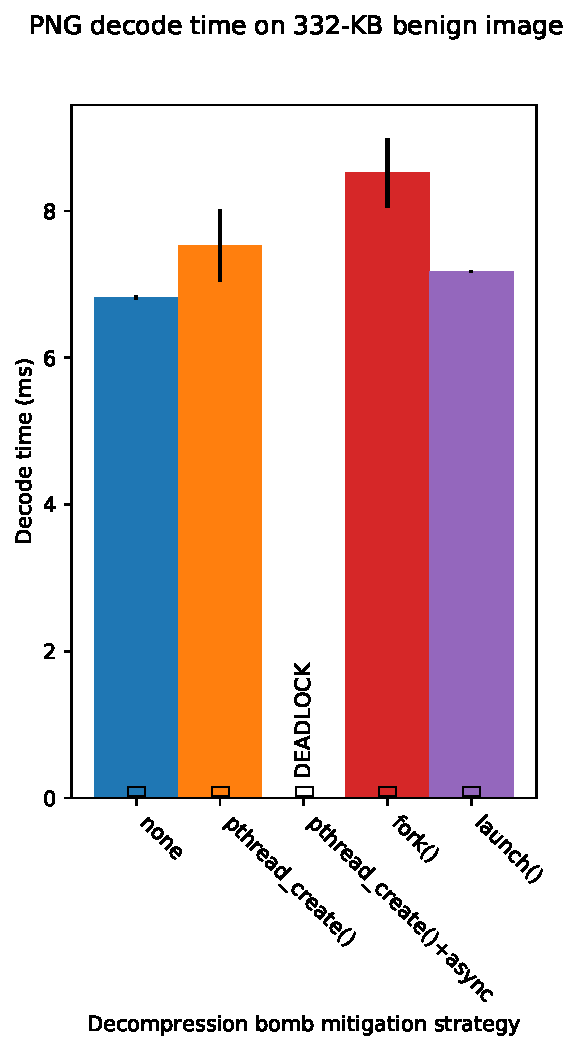
\includegraphics[width=\textwidth]{figs/cerberus2_nns16_surplus256k_mirjam}
	\subcaption{\texttt{openclipart-png} image}
	\label{fig:libpng:benign}
	\end{minipage}
%
	\begin{minipage}{\columnwidth}
	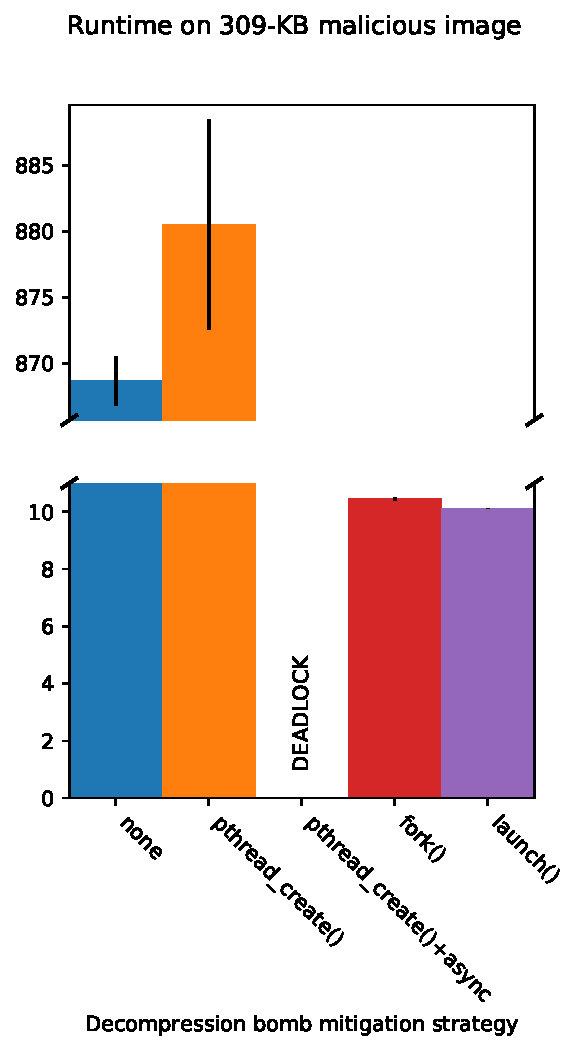
\includegraphics[width=\textwidth]{figs/cerberus2_nns16_surplus256k_10K}
	\subcaption{\texttt{bomb.codes} image}
	\label{fig:libpng:bomb}
	\end{minipage}
\caption{\textit{libpng} in-memory decode times for two different images}
\end{figure*}

Running on the benign RGB image \texttt{mirjam\_meijer\_mirjam\_mei.png} from version
\texttt{1:0.18+dfsg-15} of Debian's \texttt{openclipart-png} package showed
\texttt{launch()} to be both faster and lower-variance than the other approaches,
adding just 154 $\mu$s or 2.2\% over the baseline (Figure~\ref{fig:libpng:benign}).
Although the cost
of \texttt{fork()} was significantly higher when run with \textit{libgotcha}, we
consider this a positive result:\@ it is a reminder that the cost of \texttt{fork()}
is proportional to the number of pages the process has mapped.

Next, we tried a similarly-sized RGB decompression bomb from revision
\texttt{b726584} of \url{https://bomb.codes} (Figure~\ref{fig:libpng:bomb}):  We omit
the unmitigated measurement (to keep the graph scale from growing by an order of
magnitude), and could not obtain results for \texttt{pthread\_create()} (due to
recurring segfaults).  Here, \texttt{launch()} exceeded the deadline by just 100
$\mu$s, a figure that includes deviation due to the 100-$\mu$s preemption interval in
addition to \textit{libinger}'s own overhead.  It again had the lowest variance.

\solb{Should I have run the baseline and thread cases without \textit{libgotcha}?}
